\documentclass{article}
\usepackage{booktabs}
\usepackage{multirow}
\usepackage{multicol}
\usepackage[backend=biber,natbib=true,style=alphabetic,maxbibnames=50]{biblatex}
\addbibresource{/home/nqbh/reference/bib.bib}
\usepackage[utf8]{vietnam}
\usepackage{tocloft}

\setlength{\parindent}{0pt}


\usepackage{minted}

\usepackage{listings}
\usepackage{xcolor}

\lstset{
    language=C++,                    % Ngôn ngữ lập trình
    basicstyle=\ttfamily\footnotesize, % Cỡ chữ nhỏ hơn
    keywordstyle=\color{blue},        % Màu từ khóa
    commentstyle=\color{gray},        % Màu chú thích
    stringstyle=\color{red},          % Màu chuỗi ký tự
    numbers=left,                     % Hiển thị số dòng bên trái
    numberstyle=\tiny\color{gray},    % Định dạng số dòng
    stepnumber=1,                     % Mỗi dòng đều có số dòng
    breaklines=true,                   % Tự động xuống dòng nếu quá dài
    frame=single                      % Đóng khung mã nguồn
}

\renewcommand{\cftsecleader}{\cftdotfill{\cftdotsep}}
\usepackage[colorlinks=true,linkcolor=blue,urlcolor=red,citecolor=magenta]{hyperref}
\usepackage{amsmath,amssymb,amsthm,enumitem,float,graphicx,mathtools,tikz}
\usetikzlibrary{angles,calc,intersections,matrix,patterns,quotes,shadings}
\allowdisplaybreaks
\newtheorem{assumption}{Assumption}
\newtheorem{baitoan}{}
\newtheorem{cauhoi}{Câu hỏi}
\newtheorem{conjecture}{Conjecture}
\newtheorem{corollary}{Corollary}
\newtheorem{dangtoan}{Dạng toán}
\newtheorem{definition}{Definition}
\newtheorem{dinhly}{Định lý}
\newtheorem{dinhnghia}{Định nghĩa}
\newtheorem{example}{Example}
\newtheorem{ghichu}{Ghi chú}
\newtheorem{hequa}{Hệ quả}
\newtheorem{hypothesis}{Hypothesis}
\newtheorem{lemma}{Lemma}
\newtheorem{luuy}{Lưu ý}
\newtheorem{nhanxet}{Nhận xét}
\newtheorem{notation}{Notation}
\newtheorem{note}{Note}
\newtheorem{principle}{Principle}
\newtheorem{problem}{Problem}
\newtheorem{proposition}{Proposition}
\newtheorem{question}{Question}
\newtheorem{remark}{Remark}
\newtheorem{theorem}{Theorem}
\newtheorem{vidu}{Ví dụ}
\usepackage[left=1cm,right=1cm,top=5mm,bottom=5mm,footskip=4mm]{geometry}
\def\labelitemii{$\circ$}
\DeclareRobustCommand{\divby}{%
	\mathrel{\vbox{\baselineskip.65ex\lineskiplimit0pt\hbox{.}\hbox{.}\hbox{.}}}%
}
\setlist[itemize]{leftmargin=*}
\setlist[enumerate]{leftmargin=*}

\title{Hướng Đến Kỳ Thi Olympic Tin học Sinh Viên Toàn Quốc {\it\&} ICPC 2025} 
\author{Đặng Phúc An Khang\footnote{ E-mail: {\tt ankhangluonvuituoi@gmail.com}. Tây Ninh, Việt Nam.}}
\date{\today}

\begin{document}
\maketitle
\begin{abstract}
	Báo cáo về quá trình ôn luyện lập trình thi đấu hướng đến kỳ thi OLP Tin học Sinh viên toàn quốc {\it\&} ICPC.
	

    \begin{itemize}
        \item C{\tt/}C++ code: \url{https://github.com/GrootTheDeveloper/OLP-ICPC/tree/master/2025/C%2B%2B}.
        \item Python code: \url{}.
    \end{itemize}
    
\end{abstract}
\tableofcontents

%------------------------------------------------------------------------------%

\section{Preliminaries -- Kiến thức chuẩn bị}

\textbf{\textsf{Resources -- Tài nguyên.}}
\begin{enumerate}
	\item \cite{WANG_WU2016}. {\sc Wang \it\& Wu}. \it Data Structure Practice for Collegiate Programming Contests and Education. \url{https://github.com/GrootTheDeveloper/OLP-ICPC/blob/master/Wu_Wang2016.pdf}
    	\item \cite{WANG_WU2019}. {\sc Wang \it\& Wu}. \it Algorithm Design Practice for Collegiate Programming Contests and Education. \url{https://github.com/GrootTheDeveloper/OLP-ICPC/blob/master/Wu_Wang2019.pdf}

\end{enumerate}
Personal Critical-thinking Questions:
\begin{question}[Expanding my problem-solving approach]
What common problem-solving techniques do I tend to use, and how can I generalize them for a broader range of problems?
How can I extract key ideas from problems I have solved and apply them to unfamiliar ones?

\end{question}

\begin{question}[Connecting different concepts]
	Can I find patterns between problems I have solved and those I struggle with? Are there underlying principles between different algorithmic topics (e.g., dynamic programming, graph theory, number theory) that I can use to approach problems more creatively?
\end{question}

\begin{question}[Innovation]
	 How can I break away from my usual way of thinking and explore new approaches?
\end{question}

\begin{question}[Improving my learning process]
Which learning methods (e.g., solving harder problems, reading editorials, discussing with others) have the most impact on enhancing my creative problem-solving skills? How can I track whether my thinking process is improving?
\end{question}

%------------------------------------------------------------------------------%

\section{WANG \it\& WU 2016}
\textbf{\textsf{Resources -- Tài nguyên.}}
\begin{enumerate}
\item Link: \url{https://github.com/GrootTheDeveloper/OLP-ICPC/blob/master/Wu_Wang2016.pdf}
\item Online Judge: \url{}
\end{enumerate}


\subsection{SECTION 1: FUNDAMENTAL PROGRAMMING SKILLS}
\subsubsection{Financial Management}
Larry graduated this year and finally has a job. He’s making a lot of money, but somehow never
seems to have enough. Larry has decided that he needs to get a hold of his financial portfolio and
solve his financial problems. The first step is to figure out what’s been going on with his money.
Larry has his bank account statements and wants to see how much money he has. Help Larry by
writing a program to take his closing balance from each of the past 12 months and calculate his
average account balance.

\paragraph{Input} \mbox{} \\

The input will be 12 lines. Each line will contain the closing balance of his bank account for a particular month. Each number will be positive and displayed to the penny. No dollar sign will be included.

\paragraph{Output}\mbox{} \\

The output will be a single number, the average (mean) of the closing balances for the 12 months. It will be rounded to the nearest penny, preceded immediately by a dollar sign, and followed by the end of the line. There will be no other spaces or characters in the output.

\paragraph{Example}\mbox{} \\

\begin{table}[h]
    \centering
    \begin{tabular}{|l|r|}
        \hline
        \textbf{Sample Input} & \textbf{Sample Output} \\
        \hline
        100.00    &  \textbf{\$1581.42} \\ 
        489.12    &  \\ 
        12454.12  &  \\ 
        1234.10   &  \\ 
        823.05    &  \\ 
        109.20    &  \\ 
        5.27      &  \\ 
        1542.25   &  \\ 
        839.18    &  \\ 
        83.99     &  \\ 
        1295.01   &  \\ 
        1.75      &  \\ \hline
    \end{tabular}
\end{table}

\textit{Source}: ACM Mid-Atlantic United States 2001.

\textbf{IDs for online judges}: POJ 1004, ZOJ 1048, UVA 2362.


\paragraph{Analysis -- Phân tích bài toán} \mbox{} \\

Đề bài cho nhập 12 số thực - Dùng kiểu float/double, yêu cầu tính trung bình cộng của 12 số thực đó, làm tròn số đến 2 chữ số thập phân gần nhất (the nearest penny). Lưu ý có dấu \$ trước kết quả.

\paragraph{Program -- Chương trình} \mbox{} \\


\begin{lstlisting}
#include <bits/stdc++.h>
using namespace std;
int main() {

	double ans = 0.0;

	for (int i = 1; i <= 12; i++) {
		double x; cin >> x;
		ans += x / 12.0; 
	}

	cout << "$" << fixed << setprecision(2) << ans;
}
\end{lstlisting}



%------------------------------------------------------------------------------%

\subsubsection{Doubles}

As part of an arithmetic competency program, your students will be given randomly generated lists of 2–15 unique positive integers and asked to determine how many items in each list are twice some other item in the same list. You will need a program to help you with the grading. This program should be able to scan the lists and output the correct answer for each one. For example, given the list

{\centering 1 4 3 2 9 7 18 22 \par}

your program should answer 3, as 2 is twice 1, 4 is twice 2, and 18 is twice 9.

\paragraph{Input} \mbox{} \\

The input file will consist of one or more lists of numbers. There will be one list of numbers per
line. Each list will contain from 2 to 15 unique positive integers. No integer will be larger than 99.
Each line will be terminated with the integer 0, which is not considered part of the list. A line with
the single number –1 will mark the end of the file. The example input below shows three separate
lists. Some lists may not contain any doubles.

\paragraph{Output}\mbox{} \\

The output will consist of one line per input list, containing a count of the items that are double
some other item.

\paragraph{Example}\mbox{} \\

\begin{table}[h]
    \centering
    \begin{tabular}{|l|r|}
        \hline
        \textbf{Sample Input} & \textbf{Sample Output} \\
        \hline
        1 4 3 2 9 7 18 22 0  &  3 \\ 
        2 4 8 10 0    & 2 \\ 
        7 5 11 13 1 3 0  &  0 \\ 
        -1   &  \\ \hline
    \end{tabular}
\end{table}

\textit{Source}: ACM Mid-Central United States 2003.

\textbf{IDs for online judges}: POJ 1552, ZOJ 1760, UVA 2787.


\paragraph{Analysis -- Phân tích bài toán} \mbox{} \\

Tiếp cận phần thuật toán, nhận xét rằng nếu biến đang nhập có giá trị lẻ (tức chia lấy dư cho 2 dư 1) thì không cần xét. Vì không thể lấy 2 lần một số nguyên nào mà ra kết quả có giá trị lẻ. Ngược lại, nếu biến mang giá trị chẵn thì lưu vào CTDL cây nhị phân map. Vậy khi tìm kiếm ta chỉ cần tìm nửa giá trị của biến, và đếm số lượng tìm được. \\

Bài toán có dạng multi-testcase, mỗi bộ test kết thúc bằng số 0, và bài toán chỉ kết thúc khi gặp số 1. \\

Vậy chỉ cần vòng lặp vô hạn, đặt điều kiện: \\

- Nếu biến đang nhập mang giá trị 0, Xử lý và xuất kết quả bài toán, sau đó reset trạng thái mọi biến/CTDL ta dùng. \\
- Nếu biến đang nhập mang giá trị -1, break chương trình  

\paragraph{Program -- Chương trình} \mbox{} \\


\begin{lstlisting}
#include <bits/stdc++.h>
using namespace std;

int main() {	
	map<int, int> ma;
	vector<int>a;
	int n; int ans = 0;
	while (cin >> n) {
		if (n == -1) {
			break;
		}
		if (n == 0) {
			for (int i : a) {
				if (i % 2 == 1) continue;
				ans += ma[i / 2];
			}
			cout << ans << endl;
			ans = 0;
			ma.clear();
			a.clear();
			continue;
		}
		a.push_back(n);
		ma[n]++;
	}
}
	
\end{lstlisting}

%------------------------------------------------------------------------------%

\subsubsection{Sum of Consecutive Prime Numbers}

Some positive integers can be represented by a sum of one or more consecutive prime numbers.
How many such representations does a given positive integer have? For example, the integer 53
has two representations 5 + 7 + 11 + 13 + 17 and 53. The integer 41 has three representations:
2 + 3 + 5 + 7 + 11 + 13, 11 + 13 + 17, and 41. The integer 3 has only one representation, which is
3. The integer 20 has no such representations. Note that summands must be consecutive prime
numbers, so neither 7 + 13 nor 3 + 5 + 5 + 7 is a valid representation for the integer 20. Your
mission is to write a program that reports the number of representations for the given positive
integer.

\paragraph{Input} \mbox{} \\

The input is a sequence of positive integers, each in a separate line. The integers are between 2 and
10,000, inclusive. The end of the input is indicated by a zero.

\paragraph{Output}\mbox{} \\

The output should be composed of lines each corresponding to an input line, except the last zero.
An output line includes the number of representations for the input integer as the sum of one or
more consecutive prime numbers. No other characters should be inserted in the output.

\paragraph{Example}\mbox{} \\

\begin{table}[h]
    \centering
    \begin{tabular}{|l|r|}
        \hline
        \textbf{Sample Input} & \textbf{Sample Output} \\
        \hline
        2  &  1 \\ 
        3  &  1 \\ 
        17 &  2 \\ 
        41 &  3 \\
        20 & 0 \\
        666 & 0 \\
        12 & 1 \\ 
        53 & 2 \\
        0 & \\\hline
    \end{tabular}
\end{table}

\textit{Source}: ACM Japan 2005.

\textbf{IDs for online judges}: POJ 2739, UVA 3399.

\paragraph{Analysis -- Phân tích bài toán} \mbox{} \\

Bài toán có dạng multi-testcase với điều kiện là nhập đến khi gặp giá trị 0. \\

Tiếp cận phần thuật toán, bài toán yêu cầu với số nguyên $N$ (với $2 \leq N \leq 10000$), liệu có thể phân tích được bao nhiêu dạng tổng các số nguyên tố liên tiếp nhau. \\

Vậy, công việc đầu tiên là tạo mảng $prime$ với ý nghĩa là lưu trữ các số nguyên tố trong đoạn $[2..10000]$. Ở bước này, ta thực hiện kiểm tra số nguyên tố bằng cách thử chia từ $2$ đến $\sqrt{i}$, nếu $i$ chia hết cho bất kỳ số nào trong khoảng này thì $i$ không phải số nguyên tố. (Có thể tối ưu hơn với Sàng nguyên tố $Eratosthenes$, tuy nhiên không cần thiết lắm với bài này)\\

Tiếp theo, thay vì dùng 2 vòng for lồng nhau để xét mọi cặp chỉ số, ta sẽ sử dụng thuật toán \textbf{Two-Pointer} để đảm bảo kiểm tra hết tất cả các đoạn tổng liên tiếp một cách nhanh chóng. \\

Cách tiếp cận \textbf{Two-Pointer} được triển khai như sau: \\

- Đặt hai con trỏ \texttt{left} và \texttt{right}, bắt đầu từ đầu mảng \texttt{prime}. \\
- Dùng biến \texttt{sum} để lưu tổng các số nguyên tố trong đoạn $[left, right]$. \\
- Nếu \texttt{sum < N}, tăng \texttt{right} để mở rộng đoạn. \\
- Nếu \texttt{sum > N}, tăng \texttt{left} để thu hẹp đoạn. \\
- Nếu \texttt{sum == N}, tăng biến đếm \texttt{count}, sau đó tiếp tục dịch \texttt{left} để tìm các đoạn khác. \\

Độ phức tạp: $O(T(N^{3/2} + M))$ với $N = 10000$, $T$ là số testcase, $M$ là số lượng số nguyên tố trong đoạn $[2..10000]$. Trong đó $O(N^{3/2})$ là thời gian sinh số nguyên tố và $O(M)$ là thời gian kiểm tra các tổng liên tiếp. \\

\paragraph{Program -- Chương trình} \mbox{} \\


\begin{lstlisting}
#include <bits/stdc++.h>
using namespace std;

vector<int>primes;

int main() {
	for (int i = 2; i <= 1000; i++) {
		bool check = true;

		for (int j = 2; j <= sqrt(i); j++) {
			if (i % j == 0) {
				check = false;
				break;
			}
		}
		if (check) {
			primes.push_back(i);
		}
	}

	int N;
	while (cin >> N && N != 0) {
		int count = 0;
		int left = 0, right = 0, sum = 0;

		while (right < primes.size()) {
			if (sum < N) {
				sum += primes[right++];
			}
			else if (sum > N) {
				sum -= primes[left++];
			}
			else {
				count++;
				sum -= primes[left++];
			}
		}

		cout << count << endl;

	}
}
	
\end{lstlisting}

%------------------------------------------------------------------------------%

\subsubsection{I Think I Need a Houseboat}

Fred Mapper is considering purchasing some land in Louisiana to build his house on. In the
process of investigating the land, he learned that the state of Louisiana is actually shrinking by
50 square miles each year, due to erosion caused by the Mississippi River. Since Fred is hoping to
live in this house for the rest of his life, he needs to know if his land is going to be lost to erosion.
After doing more research, Fred has learned that the land that is being lost forms a semicircle.
This semicircle is part of a circle centered at (0, 0), with the line that bisects the circle being the X axis. Locations below the X axis are in the water. The semicircle has an area of 0 at the beginning
of year 1. \\

\begin{center}
        
\includegraphics[width=0.6\textwidth]{Figures/03.png}
\end{center}

\paragraph{Input} \mbox{} \\

The first line of input will be a positive integer indicating how many data sets will be included $(N)$. Each of the next $N$ lines will contain the $X$ and $Y$ Cartesian coordinates of the land Fred is considering. These will be floating-point numbers measured in miles. The $Y$ coordinate will be
nonnegative. $(0, 0)$ will not be given.

\paragraph{Output}\mbox{} \\

For each data set, a single line of output should appear. This line should take the form of

\begin{center} Property $N$: This property will begin eroding in year $Z$.
\end{center}
where $N$ is the data set (counting from 1) and $Z$ is the first year (start from 1) this property will be within the semicircle AT THE END OF YEAR Z. Z must be an integer. After the last data set,
this should print out “END OF OUTPUT.”


\paragraph{Example}\mbox{} \\

\begin{table}[h]
    \centering
    \begin{tabular}{|l|r|}
        \hline
        \textbf{Sample Input} & \textbf{Sample Output} \\
        \hline
           2 & Property 1: This property will begin ercoding in year 1.  \\ 
           1.0 1.0 & Property 1: This property will begin ercoding in year 20. \\ 
           25.0 0.0 & END OF OUTPUT. \\  \hline
    \end{tabular}
\end{table}

\textit{Source}: ACM Mid-Atlantic United States 2001. \\

\textit{Note}: No property will appear exactly on the semicircle boundary: it will be
either inside or outside. This problem will be judged automatically. Your
answer must match exactly, including the capitalization, punctuation,
and white space. This includes the periods at the ends of the lines. All
locations are given in miles.
\\ 
\\
\textbf{IDs for online judges}:  POJ 1005, ZOJ 1049, UVA 2363.


\paragraph{Analysis -- Phân tích bài toán} \mbox{} \\

Diện tích đất bị xói mòn 50 dặm vuông mỗi năm, và xói mòn theo dạng nửa hình tròn. Ta có công thức:\\

\begin{center}
    $S = \frac{1}{2}\pi r^2$
    $\Rightarrow{r = \sqrt{\frac{2S}{\pi}}}$
\end{center}

Với $S$ tăng đều mỗi năm 50 dặm vuông, $r$ cũng tăng theo, ta chỉ cần so sánh xem độ dài từ tâm $O$ đến điểm $(x,y)$ cần xét (bán kính $R' = \sqrt{x^2+y^2}$) có nhỏ hơn $r$ không, nếu nhỏ hơn, chỉ cần tăng $S$ (số năm tăng) đến khi $R' < r$. Đến khi đó, ta xác định được số năm cần tìm. \\ 

Có thể sử dụng kỹ thuật tìm kiếm nhị phân để tìm nhanh hơn, trong đoạn $[L..R]$, ta tìm điểm giữa $mid = (l + r) / 2$ với ý nghĩa $mid$ là số năm đã bị xói mòn, từ đó ta có được $S$ mới (diện tích nửa hình tròn sau $mid$ year), từ $S$ mới ta suy ra được $r$.\\

Nếu $r < R'$ có nghĩa là điểm $(x,y)$ vẫn nằm ngoài nửa hình tròn sau $mid$ năm. Vậy ta tiếp tục kiểm tra đoạn $[mid + 1, R]$. \\
Nếu $r >= R'$ có nghĩa là điểm $(x,y)$ đã nằm trong đường tròn sau $mid$ năm. Ta lưu kết quả $yearEnd$ tốt nhất hiện tại, và tiếp tục xét đoạn $[L..mid-1]$ xem có năm nào sớm hơn mà vẫn thỏa mãn điểm $(x,y)$ nằm trong nửa hình tròn không.

\paragraph{Program -- Chương trình} \mbox{} \\



\begin{lstlisting}
#include <bits/stdc++.h>
using namespace std;

const double PI = 3.1415926;

double calcR(double x, double y) {
	return sqrt(x * x + y * y);
}

int main() {
	int properties; cin >> properties;

	for (int property = 1; property <= properties; property++) {
		
		double x, y; cin >> x >> y;

		int yearEnd = 1;
		double S = 50.0;
		double R = sqrt(2 * S / PI);

		int l = 1;
		int r = 1e9 + 7;

		while (l <= r) {
			int mid = l + r >> 1;
			S = 50.0 * mid;
			R = sqrt(2 * S / PI);
			if (calcR(x, y) >= R) {
				l = mid + 1;
			}
			else {
				yearEnd = mid;
				r = mid - 1;
			}
		}

		cout << "Property " << property << ": This property will begin eroding in year " << yearEnd << "." << endl;
	}
	cout << "END OF FILE.";
}
\end{lstlisting}



%------------------------------------------------------------------------------%

%------------------------------------------------------------------------------%

\subsubsection{Hangover}

How far can you make a stack of cards overhang a table? If you have one card, you can create a
maximum overhang of half a card length. (We’re assuming that the cards must be perpendicular to the table.) With two cards, you can make the top card overhang the bottom one by half a
card length, and the bottom one overhang the table by a third of a card length, for a total maximum overhang of 1/2 + 1/3 = 5/6 card lengths. In general, you can make n cards overhang by
1/2 + 1/3 + 1/4 + … + 1/(n + 1) card lengths, where the top card overhangs the second by 1/2, the
second overhangs the third by 1/3, the third overhangs the fourth by 1/4, and so on, and the bottom card overhangs the table by 1/(n + 1). This is illustrated in Figure 1.2.

\begin{center}
    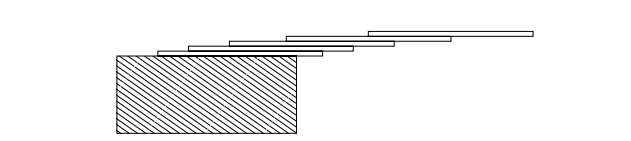
\includegraphics[width=0.6\textwidth]{Figures/04.png} \\
    \textbf{Figure 1.2 : A stack of cards overhangs a table.}
\end{center}

\paragraph{Input} \mbox{} \\
The input consists of one or more test cases, followed by a line containing the number 0.00 that
signals the end of the input. Each test case is a single line containing a positive floating-point number c whose value is at least 0.01 and at most 5.20; c will contain exactly three digits.

\paragraph{Output}\mbox{} \\
For each test case, output the minimum number of cards necessary to achieve an overhang of at
least c card lengths. Use the exact output format shown in the examples.

\paragraph{Example}\mbox{} \\

\begin{table}[h]
    \centering
    \begin{tabular}{|l|r|}
        \hline
        \textbf{Sample Input} & \textbf{Sample Output} \\
        \hline
         1.00  & 3 card(s)  \\ 
         3.71  & 61 card(s) \\ 
         0.04  & 1 card(s) \\ 
         5.19  & 273 card(s) \\ 
         0.00 & \\ \hline
    \end{tabular}
\end{table}

\textit{Source}: 

\textbf{IDs for online judges}: 


\paragraph{Analysis -- Phân tích bài toán} \mbox{} \\

Trước hết, tôi thử nháp xem rằng với bao nhiêu lá bài thì $c$ vượt qua giá trị $5.20$.

\begin{lstlisting}
	double ans = 0.00;
	for (int i = 1; i <= 10000; i++) {
		ans += 1 / (1.0 * (i + 1));
		cout << ans << " ";
		if (ans > 5.2) {
			cout << "-" << i << "-";
			break;
		}
	}
\end{lstlisting}

Kết quả cho thấy: có tối đa 276 lá bài. \\

Vậy nên, tôi tạo một mảng $f[277]$ với ý nghĩa $f[i]$ lưu tổng giá trị của $1/2 + 1/3 + 1/4 + . . . + 1/(n + 1)$. Tiếp đến, ta cần tìm chỉ số $i$ nhỏ nhất sao cho $c \leq f[i]$. Sau khi tìm được, kết quả bài toán là $i$. Vì kích thước bài toán nhỏ, ta có thể duyệt for chạy hết mảng, nếu gặp $f[i] \geq c$, ta lập tức biết được kết quả cần tìm là $i$.\\

Ở đây tôi dùng tìm kiếm nhị phân để trông có vẻ "pro" hơn.

\paragraph{Program -- Chương trình} \mbox{} \\


\begin{lstlisting}
#include <bits/stdc++.h>
using namespace std;

int main() {

	double n;
	vector<double>f(277, 0.00);

	for (int i = 1; i <= 276; i++) {
		f[i] = f[i - 1] + (1.0 / (1.0*i + 1));
	}

	while (cin >> n && n != 0.00) {
		int ans = 0;

		int l = 1, r = 276;
		while (l <= r) {
			int mid = l + r >> 1;
			if (f[mid] == n) {
				ans = mid;
				break;
			}
			if (f[mid] > n) {
				ans = mid;
				r = mid - 1;
			}
			else {
				l = mid + 1;
			}
		}

		cout << ans << " card(s)" << endl;
	}
}
\end{lstlisting}

%---------------------------------------------------------------------------------------------%


\subsubsection{Humidex}

The humidex is a measurement used by Canadian meteorologists to reflect the combined effect of heat and humidity. It differs from the heat index used in the United States in using dew point rather than relative humidity.\\
When the temperature is 30°C (86°F) and the dew point is 15°C (59°F), the humidex is 34 (note that humidex is a dimensionless number, but the number indicates an approximate temperature in Celsius). If the temperature remains 30°C and the dew point rises to 25°C (77°F), the
humidex rises to 42.3. \\
The humidex tends to be higher than the U.S. heat index at equal temperature and relative humidity. \\
The current formula for determining the humidex was developed by J.M. Masterton and F.A. Richardson of Canada’s Atmospheric Environment Service in 1979. \\
According to the Meteorological Service of Canada, a humidex of at least 40 causes “great discomfort” and above 45 is “dangerous.” When the humidex hits 54, heat stroke is imminent. \\
The record humidex in Canada occurred on June 20, 1953, when Windsor, Ontario, hit 52.1. (The residents of Windsor would not have known this at the time, since the humidex had yet to be invented.) More recently, the humidex reached 50 on July 14, 1995, in both Windsor and Toronto.\\

The humidex formula is as follows: 

\begin{align*}
    \text{humidex} &= \text{temperature} + h \\
    h &= (0.5555) \cdot (e - 10.0) \\
    e &= 6.11 \times \exp \left( 5417.7530 \left( \frac{1}{273.16} - \frac{1}{\text{dewpoint} + 273.16} \right) \right)
\end{align*}

where \( \exp(x) \) is \( 2.718281828 \) raised to the exponent \( x \). \\

While humidex is just a number, radio announcers often announce it as if it were the temperature, for example, “It’s 47° out there … with the humidex.” Sometimes weather reports give the temperature and dew point, or the temperature and humidex, but rarely do they report all three
measurements. Write a program that, given any two of the measurements, will calculate the third.\\
You may assume that for all inputs, the temperature, dew point, and humidex are all between
–100°C and 100°C.


\paragraph{Input} \mbox{} \\

Input will consist of a number of lines. Each line except the last will consist of four items separated
by spaces: a letter, a number, a second letter, and a second number. Each letter specifies the meaning of the number that follows it and will be either T, indicating temperature; D, indicating dew
point; or H, indicating humidex. The last line of input will consist of the single letter E

\paragraph{Output}\mbox{} \\

For each line of input except the last, produce one line of output. Each line of output should have
the form:
\begin{center}
T number D number H number
\end{center}
where the three numbers are replaced with the temperature, dew point, and humidex. Each value
should be expressed rounded to the nearest tenth of a degree, with exactly one digit after the decimal point. All temperatures are in degrees Celsius

\paragraph{Example}\mbox{} \\

\begin{table}[h]
    \centering
    \begin{tabular}{|l|r|}
        \hline
        \textbf{Sample Input} & \textbf{Sample Output} \\
        \hline
         T 30 D 15   & T 30.0 D 15.0 H 34.0  \\ 
         T 30.0 D 25.0   & T 30.0 D 25.0 H 42.3 \\ 
         E   &  \\ 
            &  \\ \hline
    \end{tabular}
\end{table}

\textit{Source}: Waterloo Local Contest, July 14, 2007

\textbf{IDs for online judges}: POJ 3299.


\paragraph{Analysis -- Phân tích bài toán} \mbox{} \\


\paragraph{Program -- Chương trình} \mbox{} \\


\begin{lstlisting}

\end{lstlisting}



%---------------------------------------------------------------------------------------------%

\subsubsection{Sum}

Your task is to find the sum of all integer numbers lying between 1 and $N$ inclusive.

\paragraph{Input} \mbox{} \\

The input consists of a single integer $N$ that is not greater than 10,000 by its absolute value.

\paragraph{Output}\mbox{} \\

Write a single integer number that is the sum of all integer numbers lying between $1$ and $N$ inclusive.

\paragraph{Example}\mbox{} \\

\begin{table}[h]
    \centering
    \begin{tabular}{|l|r|}
        \hline
        \textbf{Sample Input} & \textbf{Sample Output} \\
        \hline
        -3 & -5  \\ 
            &  \\ \hline
    \end{tabular}
\end{table}

\textit{Source}: ACM 2000, Northeastern European Regional Programming Contest (test tour). \\

\textbf{IDs for online judges}: Ural 1068. \\

\textit{Hint}: Based on the summation formula of arithmetic progression s = 1 + 2 + … N, if N is an integer larger than 0, then s = [(1 + N)/2]*N; otherwise, s = [(1 – N)/2]*N + 1.


\paragraph{Analysis -- Phân tích bài toán} \mbox{} \\

Công thức tính tổng dãy số cách đều {1, 2, 3, ... , $N$} là $S = N * ( N + 1) / 2$.\\

Nếu $N \leq 0$, ta cần tính $S$ từ $1$ đến $-N$, sau đó kết quả sẽ là $-S+1$. \\

Nếu $N > 0$, ta đơn giản là tính $S$ dựa theo công thức thôi. \\

\paragraph{Program -- Chương trình} \mbox{} \\


\begin{lstlisting}

#include <bits/stdc++.h>
using namespace std;

int main() {

	int n; cin >> n;
	if (n <= 0) {
		n = -n;
		cout << -n * (n + 1) / 2 + 1;
	}
	else {
		cout << n * (n + 1) / 2;
	}
}

\end{lstlisting}


%---------------------------------------------------------------------------------------------%

\subsubsection{Specialized Four-Digit Numbers}

Find and list all four-digit numbers in decimal notation that have the property that the sum of their four digits equals the sum of their digits when represented in hexadecimal (base 16) notation and also equals the sum of their digits when represented in duodecimal (base 12) notation. \\

For example, the number 2991 has the sum of (decimal) digits 2 + 9 + 9 + 1 = 21. Since 2991 = 1*1728 + 8*144 + 9*12 + 3, its duodecimal representation is 189312, and these digits also sum up to 21. But in hexadecimal, 2991 is BAF16, and 11 + 10 + 15 = 36, so 2991 should be rejected by your program.\\

The next number (2992), however, has digits that sum to 22 in all three representations (including BB016), so 2992 should be on the listed output. (We don’t want decimal numbers with fewer than four digits—excluding leading zeros—so that 2992 is the first correct answer.) \\

\paragraph{Input} \mbox{} \\

There is no input for this problem.

\paragraph{Output}\mbox{} \\

Your output is to be 2992 and all larger four-digit numbers that satisfy the requirements (in strictly increasing order), each on a separate line, with no leading or trailing blanks, ending with a new-line character. There are to be no blank lines in the output. The first few lines of the output are shown below:

\paragraph{Example}\mbox{} \\

\begin{table}[h]
    \centering
    \begin{tabular}{|l|r|}
        \hline
        \textbf{Sample Input} & \textbf{Sample Output} \\
        \hline
            & 2992  \\ 
            & 2993 \\ 
            & 2994 \\ 
            & 2995 \\ 
            & 2996\\ 
            & ... \\ \hline
    \end{tabular}
\end{table}

\textit{Source}: ACM Pacific Northwest 2004.

\textbf{IDs for online judges}: POJ 2196, ZOJ 2405, UVA
3199.


\paragraph{Analysis -- Phân tích bài toán} \mbox{} \\

Với hệ cơ số $N$ bất kì, ta có thể tính tổng các chữ số bằng cách: \\

\begin{lstlisting}

int calc(int n, int base) {
	int ans = 0;
	while (n) {
		ans += n % base;
		n /= base;
	}
	return ans;
}

\end{lstlisting}

Trong đó, $base$ là hệ cơ số, $n$ là số nguyên cần tính.


\paragraph{Program -- Chương trình} \mbox{} \\


\begin{lstlisting}

#include <bits/stdc++.h>
using namespace std;

int calc(int n, int base) {
	int ans = 0;
	while (n) {
		ans += n % base;
		n /= base;
	}
	return ans;
}

int main() {

	for (int i = 2991; i <= 9999; i++) {
		if (calc(i, 10) == calc(i, 16) && calc(i, 10) == calc(i, 12)) {
			cout << i << endl;
		}
	}
}


\end{lstlisting}

%---------------------------------------------------------------------------------------------%

\subsubsection{Quicksum}

A checksum is an algorithm that scans a packet of data and returns a single number. The idea
is that if the packet is changed, the checksum will also change, so checksums are often used for
detecting transmission errors, validating document contents, and in many other situations where it is necessary to detect undesirable changes in data. \\

For this problem, you will implement a checksum algorithm called quicksum. A quicksum packet allows only uppercase letters and spaces. It always begins and ends with an uppercase letter. Otherwise, spaces and letters can occur in any combination, including consecutive spaces. \\

A quicksum is the sum of the products of each character’s position in the packet times the character’s value. A space has a value of zero, while letters have a value equal to their position in the alphabet. So, A = 1, B = 2, and so on, through Z = 26. Here are example quicksum calculations
for the packets “ACM” and “MID CENTRAL”: \\

ACM: 1*1 + 2*3 + 3*13 = 46 \\

MID CENTRAL: 1*13 + 2*9 + 3*4 + 4*0 + 5*3 + 6*5 + 7*14 + 8*20 + 9*18 + 10*1 + 11*12 = 650

\paragraph{Input} \mbox{} \\

The input consists of one or more packets followed by a line containing only \# that signals the end of the input. Each packet is on a line by itself, does not begin or end with a space, and contains from 1 to 255 characters.
.

\paragraph{Output}\mbox{} \\

For each packet, output its quicksum on a separate line in the output.

\paragraph{Example}\mbox{} \\

\begin{table}[h]
    \centering
    \begin{tabular}{|l|r|}
        \hline
        \textbf{Sample Input} & \textbf{Sample Output} \\
        \hline
        ACM   &  46  \\ 
        MID CENTRAL  & 650 \\ 
        REGIONAL PROGRAMMING CONTEST & 4690 \\ 
        CONTEST    & 49 \\ 
        ACN    &  75 \\ 
        A C M    &  14\\ 
        BBC     &   15  \\
        $\#$& \\ \hline
    \end{tabular}
\end{table}

\textit{Source}: ACM Mid-Central United States 2006.

\textbf{IDs for online judges}: POJ 3094, ZOJ 2812, UVA 3594.


\paragraph{Analysis -- Phân tích bài toán} \mbox{} \\

Với các ký tự ['A'..'Z'] ta chuyển về [1..26]. Để thực hiện, ta cần xét kí tự $c$ thuộc đoạn ['A'..'Z'], sau đó ta trừ 'A' (mã ASCII) cho $c$ để dịch về [0..25] và cộng 1 để trở thành đoạn [1..26]. \\

Sample Input trong Example bị thiếu:\\
\textbf{Gốc:} REGIONAL PROGRAMMING = 4690 (thực tế là = $2240$). \\
\textbf{Sửa lại:} REGIONAL PROGRAMMING CONTEST = 4960 (chuẩn với ví dụ).

\paragraph{Program -- Chương trình} \mbox{} \\


\begin{lstlisting}

#include <bits/stdc++.h>
using namespace std;
	
int main() {
	
	string s;
	while (getline(cin, s) && s != "#") {
		int ans = 0;
		for (int i = 0; i < s.size(); i++) {
			if (s[i] == ' ') continue;
			ans += (i + 1) * (s[i] - 'A' + 1);
		}
		cout << ans << endl;
	}

}

\end{lstlisting}

%---------------------------------------------------------------------------------------------%

\subsubsection{A Contesting Decision}

Judging a programming contest is hard work, with demanding contestants, tedious decisions, and monotonous work—not to mention the nutritional problems of spending 12 hours with only donuts, pizza, and soda for food. Still, it can be a lot of fun.\\
Software that automates the judging process is a great help, but the notorious unreliability of some contest software makes people wish that something better were available. You are part of a group trying to develop better, open-source, contest management software, based on the principle of modular design. \\
Your component is to be used for calculating the scores of programming contest teams and determining a winner. You will be given the results from several teams and must determine the winner. \\

\textbf{Scoring}\\
There are two components to a team’s score. The first is the number of problems solved. The second is penalty points, which reflect the amount of time and incorrect submissions made before the problem is solved. For each problem solved correctly, penalty points are charged equal to the time
at which the problem was solved plus 20 minutes for each incorrect submission. No penalty points are added for problems that are never solved. \\

So if a team solved problem 1 on their second submission at 20 minutes, they are charged 40 penalty points. If they submit problem 2 three times, but do not solve it, they are charged no penalty points. If they submit problem 3 once and solve it at 120 minutes, they are charged 120 penalty points. Their total score is two problems solved with 160 penalty points. \\

The winner is the team that solves the most problems. If teams tie for solving the most problems, then the winner is the team with the fewest penalty points.


\paragraph{Input} \mbox{} \\

For the programming contest your program is judging, there are four problems. You are guaranteed that the input will not result in a tie between teams after counting penalty points. \\

\textit{Line 1: < nTeams >}\\
\textit{Line 2: n+1 < Name > < p1Sub > < p1Time > < p2Sub > < p2Time > …< p4Time >}\\ \\
The first element on the line is the team name, which contains no white space. Following that,
for each of the four problems, is the number of times the team submitted a run for that problem
and the time at which it was solved correctly (both integers). If a team did not solve a problem,
the time will be zero. The number of submissions will be at least one if the problem was solved.

\paragraph{Output}\mbox{} \\

The output consists of a single line listing the name of the team that won, the number of problems
they solved, and their penalty points.

\paragraph{Example}\mbox{} \\

\begin{table}[h]
    \centering
    \begin{tabular}{|l|r|}
        \hline
        \textbf{Sample Input} & \textbf{Sample Output} \\
        \hline
        4 &  Penguins 3 475 \\ 
        Stars 2 20 5 0 4 190 3 220   &  \\ 
        Rockets 5 180 1 0 2 0 3 100    &  \\ 
        Penguins 1 15 3 120 1 300 4 0    &  \\ 
        Marsupials 9 0 3 100 2 220 3 80    &  \\ 
            &  \\ \hline
    \end{tabular}
\end{table}

\textit{Source}: ACM Mid-Atlantic 2003.

\textbf{IDs for online judges}: POJ 1581, ZOJ 1764, UVA 2832.


\paragraph{Analysis -- Phân tích bài toán} \mbox{} \\

Mấu chốt quyết định đầu tiên là số bài giải được, có nghĩa là $Time > 0$ là nhiều nhất. Sau đó mới xét đến $Penalty$.\\

Bài toán chỉ để kiểm tra khả năng quản lý biến chứ không có gì khó khăn.

\paragraph{Program -- Chương trình} \mbox{} \\

\begin{lstlisting}

#include <bits/stdc++.h>
using namespace std;
	

struct problem {
	int sub, time;
};
struct team {
	string name;
	problem prob[4];
};
int main() {
	
	int n; cin >> n;

	vector<team>a(n);
	for (int i = 0; i < n; i++) {
		cin >> a[i].name;
		for (int j = 0; j < 4; j++) {
			cin >> a[i].prob[j].sub >> a[i].prob[j].time;
		}
	}


	int maxSolve = 0;
	int maxPenalty = 0;
	string maxName;


	for (int i = 0; i < n; i++) {
		int currentPenalty = 0;
		int currentSolve = 0;
		string currentName = a[i].name;
		for (int j = 0; j < 4; j++) {
			currentPenalty += (a[i].prob[j].time > 0 ? a[i].prob[j].time + (20 * (a[i].prob[j].sub <= 1 ? 0 : a[i].prob[j].sub - 1)) : 0);
			currentSolve += (a[i].prob[j].time > 0 ? 1 : 0);
		}

		if (currentSolve > maxSolve) {
			maxSolve = currentSolve;
			maxPenalty = currentPenalty;
			maxName = currentName;
		}
		else if (currentSolve == maxSolve) {
			if (currentPenalty < maxPenalty) {
				maxSolve = currentSolve;
				maxPenalty = currentPenalty;
				maxName = currentName;
			}
		}
	}
	cout << maxName << " " << maxSolve << " " << maxPenalty;
}

\end{lstlisting}

%---------------------------------------------------------------------------------------------%

\subsubsection{Dirichlet’s Theorem on Arithmetic Progressions}

If a and d are relatively prime positive integers, the arithmetic sequence beginning with a and increasing by d, that is, a, a +  d, a + 2d, a + 3d, a + 4d, …, contains infinitely many prime numbers. This fact is known as Dirichlet’s theorem on arithmetic progressions, which had been conjectured by Johann Carl Friedrich Gauss (1777–1855) and was proved by Johann Peter Gustav Lejeune Dirichlet (1805–1859) in 1837. \\

For example, the arithmetic sequence beginning with 2 and increasing by 3, that is, \\ 2, 5, 8, 11, 14, 17, 20, 23, 26, 29, 32, 35, 38, 41, 44, 47, 50, 53, 56, 59, 62, 65, 68, 71, 74, 77, 80, 83, 86, 89, 92, 95, 98, …. \\

contains infinitely many prime numbers:

\begin{center}
2, 5, 11, 17, 23, 29, 41, 47, 53, 59, 71, 83, 89, …
\end{center}
Your mission, should you choose to accept it, is to write a program to find the nth prime number in this arithmetic sequence for given positive integers $a, d,$ and $n$.

\paragraph{Input} \mbox{} \\

The input is a sequence of data sets. A data set is a line containing three positive integers $a, d,$ and $n$ separated by a space. a and d are relatively prime. You may assume $a \leq 9307$, $d \leq 346$, and $n \leq 210$. \\
The end of the input is indicated by a line containing three zeros separated by a space. It is not a data set.

\paragraph{Output}\mbox{} \\

The output should be composed of as many lines as the number of the input data sets. Each line should contain a single integer and should never contain extra characters. \\

The output integer corresponding to a data set $a, d, n$ should be the nth prime number among those contained in the arithmetic sequence beginning with a and increasing by $d$. \\

For your information, it is known that the result is always less than 106 (1 million) under this input condition.


\paragraph{Example}\mbox{} \\

\begin{table}[h]
    \centering
    \begin{tabular}{|l|r|}
        \hline
        \textbf{Sample Input} & \textbf{Sample Output} \\
        \hline
        367 186 151 & 92809 \\
        179 10 203 & 6709 \\
        271 37 39 & 12037 \\
        103 230 1 & 103 \\
        27 104 185 & 93523 \\
        253 50 85 & 14503 \\
        1 1 1 & 2 \\
        9075 337 210 & 899429 \\
        307 24 79 & 5107 \\
        331 221 177 & 412717 \\
        259 170 40 & 22699 \\
        269 58 102 & 25673 \\
        0 0 0 & \\ 
        \hline
    \end{tabular}
\end{table}

\textit{Source}: ACM Japan 2006, Domestic.

\textbf{IDs for online judges}: POJ 3006.


\paragraph{Analysis -- Phân tích bài toán} \mbox{} \\

Với $a \leq 9307, d \leq 346, n \leq 210,$ số nguyên tố lớn nhất có thể xuất hiện trong giới hạn này là: 469487. \\

Kiểm tra bằng đoạn code:\\

\begin{lstlisting}
#include <bits/stdc++.h>
using namespace std;
	
bool check(int n) {
	if (n == 2 || n == 3) return true;
	for (int i = 2; i * i <= n; i++) {
		if (n % i == 0) return false;
	}
	return true;
}

int main(){
	int a = 9307;
	int d = 346;
	int cnt = 0;
	int i = 0;
	for (; cnt < 210;) {
		if (check(a + i * d)) {
			cout << a + i * d << " ";
			cnt++;
		}
		i++;
	}
}
\end{lstlisting}

dễ dàng thấy được đúng là vậy. Vậy để tối ưu tốc độ, ta dùng sàng nguyên tố Eratosthenes với giới hạn là 469487 + 1 (0-index-based).

Việc còn lại chỉ cần kiểm tra số nguyên tố thứ $n$ trong dãy số được cho.


\paragraph{Program -- Chương trình} \mbox{} \\


\begin{lstlisting}

#include <bits/stdc++.h>
using namespace std;
	
int maxPrimeNumber = 469487;
vector<bool> prime(maxPrimeNumber + 1, true);

void sieve() {
	prime[0] = prime[1] = false;
	for (int i = 2; i * i <= maxPrimeNumber; i++) {
		if (prime[i]) {
			for (int j = i * i; j <= maxPrimeNumber; j += i) {
				prime[j] = false;
			}
		}
	}
}

int main(){
	sieve();
	int a, d, n; 
	while (cin >> a && a != 0 && cin >> d >> n) {
		int number = 0;
		int index = 0;
		int result = 0;
		while (number < n) {
			if (prime[a + index * d] == true) {
				number++;
				result = a + index * d;
			}
			index++;
		}
		
		cout << result << endl;
	}
}

\end{lstlisting}

%---------------------------------------------------------------------------------------------%

\subsubsection{The Circumference of the Circle}

To calculate the circumference of a circle seems to be an easy task—provided you know its diameter. But what if you don’t? \\
You are given the Cartesian coordinates of three noncollinear points in the plane. \\
Your job is to calculate the circumference of the unique circle that intersects all three
points.

\paragraph{Input} \mbox{} \\

The input file will contain one or more test cases. Each test case consists of one line containing six real
numbers, $x_1, y_1, x_2, y_2, x_3, y_3$, representing the coordinates of the three points. The diameter of the circle
determined by the three points will never exceed 1 million. Input is terminated by the end of the file.

\paragraph{Output}\mbox{} \\

For each test case, print one line containing one real number telling the circumference of the circle
determined by the three points. The circumference is to be printed accurately rounded to two decimals. The value of $\pi$ is approximately 3.141592653589793.


\paragraph{Example}\mbox{} \\

\begin{table}[h]
    \centering
    \begin{tabular}{|l|r|}
        \hline
        \textbf{Sample Input} & \textbf{Sample Output} \\
        \hline
        0.0 –0.5 0.5 0.0 0.0 0.5    & 3.14  \\ 
        0.0 0.0 0.0 1.0 1.0 1.0    & 4.44 \\ 
        5.0 5.0 5.0 7.0 4.0 6.0    & 6.28 \\ 
        0.0 0.0 –1.0 7.0 7.0 7.0    & 31.42 \\ 
        50.0 50.0 50.0 70.0 40.0 60.0 & 62.83  \\ 
        0.0 0.0 10.0 0.0 20.0 1.0    & 632.24 \\ 
        0.0 –500000.0 500000.0 0.0 0.0 & 3141592.65\\
        500000.0 & \\
         \hline
    \end{tabular}
\end{table}

\textit{Source}: : Ulm Local Contest 1996.

\textbf{IDs for online judges}: POJ 2242, ZOJ 1090.


\paragraph{Analysis -- Phân tích bài toán} \mbox{} \\

Chu vi của đường tròn: $C = 2 \pi R$\\
Trong đó:
\begin{itemize}
    \item $R$ là bán kính đường tròn
    \item $\pi = 3.141592653589793$ 
\end{itemize}

Ta cần tìm bán kính của đường tròn ngoại tiếp tam giác 3 điểm $(x_1,y_1), (x_2,y_2), (x_3,y_3)$. Công thức tính diện tích của đường tròn ngoại tiếp tam giác là: \\

\begin{center}
    $A = \frac{1}{2}|x_1(y_2-y_3) + x_2(y_3-y_1) + x_3(y_1-y_2)$|.    
\end{center}

Sau đó, tìm bán kính của đường tròn ngoại tiếp bằng công thức:

\begin{center}
    $R = \frac{\sqrt{(x_2-x_1)^2 +(y_2-y_1)^2}.\sqrt{(x_3-x_1)^2+(y_3-y_1)^2}.\sqrt{(x_2-x_3)^2+(y_2-y_3)^2}}{4A}$
\end{center}

Cuối cùng là tìm chu vi của đường tròn.

\paragraph{Program -- Chương trình} \mbox{} \\


\begin{lstlisting}

#include <bits/stdc++.h>
using namespace std;

struct point {
	double x, y;
};

double pw(double x) {
	return x * x;
}

double triangle(point p1, point p2, point p3) {
	return 0.5 * abs(p1.x * (p2.y - p3.y) + p2.x * (p3.y - p1.y) + p3.x * (p1.y - p2.y));
}

double R(point p1, point p2, point p3) {
	double ans = (sqrt(pw(p1.x - p2.x) + pw(p1.y - p2.y)) * sqrt(pw(p1.x - p3.x) + pw(p1.y - p3.y)) * sqrt(pw(p2.x - p3.x) + pw(p2.y - p3.y)));
	ans /= 4.0 * triangle(p1, p2, p3);
	return ans;
}

const double pi = 3.141592653589793;

int main(){
	point p1, p2, p3;
	while (cin >> p1.x >> p1.y >> p2.x >> p2.y >> p3.x >> p3.y) {
		double r = R(p1, p2, p3);
		double c = 2 * pi * r;
		cout << fixed << setprecision(2) << c << endl;
	}
}

\end{lstlisting}

%---------------------------------------------------------------------------------------------%

\subsubsection{Vertical Histogram}

Write a program to read four lines of uppercase (i.e., all CAPITAL LETTERS) text input (no more than 72 characters per line) from the input file and print a vertical histogram that shows how many times each letter (but not blanks, digits, or punctuation) appears in the all-uppercase input.
Format your output exactly as shown.

\paragraph{Input} \mbox{} \\

Lines 1–4: Four lines of uppercase text, no more than 72 characters per line.


\paragraph{Output}\mbox{} \\

Lines 1–?: Several lines with asterisks and spaces followed by one line with the uppercase alphabet separated by spaces. Do not print unneeded blanks at the end of any line. Do not print any leading blank lines.

\paragraph{Example}\mbox{} \\
\begin{center}
        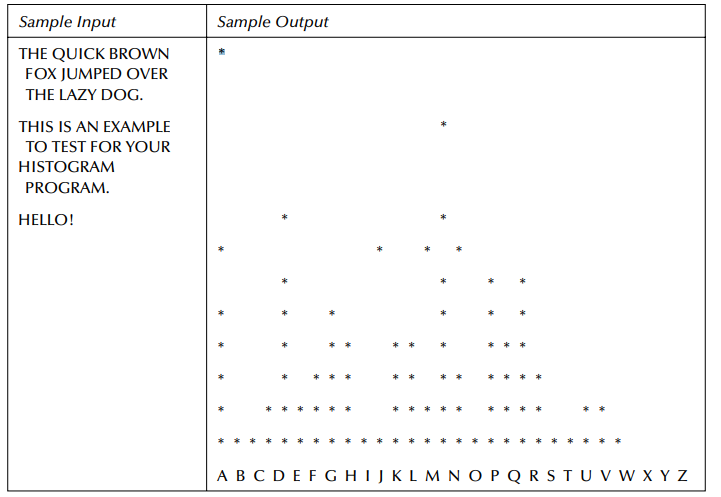
\includegraphics[width=0.6\textwidth]{Figures/05.png}
\end{center}

\textit{Source}: USACO, February 2003, Orange.

\textbf{IDs for online judges}: POJ 2136.


\paragraph{Analysis -- Phân tích bài toán} \mbox{} \\

Nhìn vào \textbf{Example}, ta thấy được tần suất ký tự xuất hiện ở các dòng tăng dần về dưới. Vậy cần $Priority$ $Queue$ quản lý tần suất các ký tự xuất hiện. \\

Thuật toán như sau: với các ký tự có lần xuất hiện cao nhất hiện tại, ta cho chúng nằm cùng 1 hàng. Sau đó đưa nó vào lại Priority Queue với lần xuất hiện hiện tại trừ đi 1, tất nhiên là nếu lần xuất hiện hiện tại > 1.

\paragraph{Program -- Chương trình} \mbox{} \\


\begin{lstlisting}
#include <bits/stdc++.h>
using namespace std;

int main(){
	string s[4];
	for (int i = 0; i < 4; i++) {
		cin >> s[i];
	}
	vector<int>character(26, 0);
	priority_queue<pair<int, char>> pq;

	for (int i = 0; i < 4; i++) {
		for (auto c : s[i]) {
			character[c - 'A']++;
		}
	}
	int maxSize = *max_element(character.begin(), character.end());

	vector<vector<char>> show(maxSize, vector<char>(26, ' '));

	for (int i = 0; i < 26; i++) {
		if (character[i] == 0) continue;
		pq.push({ character[i], i});
	}
	int idx = 0;

	while (pq.empty() == false) {
		auto [Len, C] = pq.top();
		pq.pop();
		show[idx][C] = '*';
		while (pq.empty() == false && pq.top().first == Len) {
			auto [sLen, sC] = pq.top();
			show[idx][sC] = '*';
			pq.pop();
			if (sLen == 1) continue;
			pq.push({ sLen - 1, sC });
		}
		idx++;
		if (Len == 1) continue;
		pq.push({ Len - 1, C });
	}
	

	for (int i = 0; i < maxSize; i++) {
		for (int j = 0; j < 26; j++) {
			cout << show[i][j] << "  ";
		}
		cout << endl << endl;
	}
	for (char C = 'A'; C <= 'Z'; C++) {
		cout << C << "  ";
	}
}
\end{lstlisting}

%---------------------------------------------------------------------------------------------%

\subsubsection{Ugly Numbers}

Ugly numbers are numbers whose only prime factors are 2, 3, or 5. The sequence 1, 2, 3, 4, 5, 6, 8, 9, 10, 12, … shows the first 10 ugly numbers. By convention, 1 is included. \\
Given the integer n, write a program to find and print the nth ugly number.

\paragraph{Input} \mbox{} \\

Each line of the input contains a positive integer n $(n \leq 1500)$. Input is terminated by a line with n = 0.

\paragraph{Output}\mbox{} \\
For each line, output the $n$th ugly number. Don’t deal with the line with n = 0.


\paragraph{Example}\mbox{} \\

\begin{table}[h]
    \centering
    \begin{tabular}{|l|r|}
        \hline
        \textbf{Sample Input} & \textbf{Sample Output} \\
        \hline
        1 & 1  \\ 
        2  & 2 \\ 
        9   & 10 \\ 
        0   &  \\  \hline
    \end{tabular}
\end{table}

\textit{Source}: New Zealand 1990, Division I.

\textbf{IDs for online judges}: POJ 1338, UVA 136.


\paragraph{Analysis -- Phân tích bài toán} \mbox{} \\

Số xấu quắc là số khi phân tích thừa số nguyên tố, các thừa số nguyên tố chỉ thuộc $[2,3,5]$. Vậy chỉ cần chia nó cho 2, 3, 5 (nếu chia được), sau khi chia xong, nếu số = 1 thì đương nhiên nó được tạo chỉ từ các ước số $[2,3,5]$. \\

Số 1 là ngoại lệ.

\paragraph{Program -- Chương trình} \mbox{} \\


\begin{lstlisting}

#include <bits/stdc++.h>
using namespace std;

int main(){
	int n;

	vector<int> uglyNumber;
	for (int i = 1; i <= 1500; i++) {
		int number = i;
		while (number % 2 == 0) {
			number /= 2;
		}
		while (number % 3 == 0) {
			number /= 3;
		}

		while (number % 5 == 0) {
			number /= 5;
		}
		if (number == 1) uglyNumber.push_back(i);
	}

	while (cin >> n && n != 0) {
		n--;
		cout << uglyNumber[n] << endl;
	}
}
\end{lstlisting}

%---------------------------------------------------------------------------------------------%

\subsubsection{Number Sequence}

A single positive integer i is given. Write a program to find the digit located in the position i in the sequence of number groups $S_1,S_2 …S_k$. Each group $S_k$ consists of a sequence of positive integer numbers ranging from 1 to $k$, written one after another.\\
For example, the first 80 digits of the sequence are as follows: \\
11212312341234512345612345671234567812345678912345678910123456789101112345678910
\paragraph{Input} \mbox{} \\

The first line of the input file contains a single integer t $(1 \leq t \leq 10)$, the number of test cases, followed by one line for each test case. The line for a test case contains the single integer i $(1 \leq i \leq 2147483647)$.

\paragraph{Output}\mbox{} \\

There should be one output line per test case containing the digit located in the position i.

\paragraph{Example}\mbox{} \\

\begin{table}[h]
    \centering
    \begin{tabular}{|l|r|}
        \hline
        \textbf{Sample Input} & \textbf{Sample Output} \\
        \hline
         2   & 2  \\ 
         8  &  2 \\ 
         3  &  \\ \hline
    \end{tabular}
\end{table}

\textit{Source}: ACM Tehran 2002, First Iran Nationwide Internet Programming Contest.

\textbf{IDs for online judges}: POJ 1019, ZOJ 1410


\paragraph{Analysis -- Phân tích bài toán} \mbox{} \\

\textbf{Thuật toán ngây thơ} là cho 1 chuỗi $S$ và $T$ ban đầu rỗng, duyệt idx = 1 tăng dần, cộng dồn $idx$ hiện tại vào chuỗi $T$ (tất nhiên là $idx$ đã chuyển sang dạng chuỗi), sau đó cộng dồn $T$ vào $S$, lặp đến khi nào độ dài chuỗi lớn hơn vị trí $i$ cần tìm. Kết quả là: $S[n-1]$\\

Có nghĩa là:

\begin{lstlisting}
    int T; 
	while (T--) {
		int n; cin >> n;
		string s, t;
		for (int i = 1; ; i++) {
			if (s.size() + to_string(i).size() > n) {
				break;
			}
			t += to_string(i);
			s += t;
			cout << s << endl;

		}
		cout << s[n - 1] << endl;
	}
\end{lstlisting}

Tôi gọi đây là thuật toán ngây thơ vì giới hạn bài toán lên đến $2^{63} - 1$ quá lớn, chuỗi trong C++ không thể chứa nổi.\\

Thuật toán chuẩn thì chịu.

\paragraph{Program -- Chương trình} \mbox{} \\


\begin{lstlisting}

\end{lstlisting}

%---------------------------------------------------------------------------------------------%
\subsection{SECTION 2: SIMPLE SIMULATION}
%------------------------------------------------------------------------------%

\subsubsection{Speed Limit}

Bill and Ted are taking a road trip. But the odometer in their car is broken, so they don’t know how many miles they have driven. Fortunately, Bill has a working stopwatch, so they can record their speed and the total time they have driven. Unfortunately, their record-keeping strategy is a little odd, so they need help computing the total distance driven. You are to write a program to do this computation.
For example, if their log shows\\

\begin{table}[h]
    \centering
    \begin{tabular}{|l|r|}
        \hline
        \textbf{Speed in Miles per Hour} & \textbf{Total Elapsed Time in Hours} \\
        \hline
        20  & 2  \\ \hline
        30  & 6 \\ \hline
        10  & 7 \\  \hline
    \end{tabular}
\end{table}

this means they drove 2 hours at 20 miles per hour, then 6 – 2 = 4 hours at 30 miles per hour, then 7 – 6 = 1 hour at 10 miles per hour. The distance driven is then (2)(20) + (4)(30) + (1)(10) = 40 + 120 + 10 = 170 miles. Note that the total elapsed time is always since the beginning of the trip, not since the previous entry in their log.

\paragraph{Input} \mbox{} \\

The input consists of one or more data sets. Each set starts with a line containing an integer $n$, $1 \leq n \leq 10$, followed by $n$ pairs of values, one pair per line. The first value in a pair, $s$, is the speed in miles per hour, and the second value, $t$, is the total elapsed time. Both s and t are integers, $1 \leq s \leq 90$ and $1 \leq t \leq 12$. The values for $t$ are always in strictly increasing order. A value of $–1$ for $n$ signals the end of the input.

\paragraph{Output}\mbox{} \\

For each input set, print the distance driven, followed by a space, followed by the word miles.


\paragraph{Example}\mbox{} \\

\begin{table}[h]
    \centering
    \begin{tabular}{|l|r|}
        \hline
        \textbf{Sample Input} & \textbf{Sample Output} \\
        \hline
         3   & 170 miles  \\ 
         20 2   & 180 miles \\ 
        30 6  &  90 miles \\ 
     10 7   &  \\ 
       2     &  \\ 
         60 1   &  \\
        30 5     &  \\ 
        4      &  \\ 
        15 1       &  \\ 
        25 2        &  \\ 
         30 3   &  \\ 
        10 5        &  \\
        -1  &  \\ 
                  \hline
    \end{tabular}
\end{table}

\textit{Source}: ACM Mid-Central United States 2004

\textbf{IDs for online judges}: POJ 2017, ZOJ 2176, UVA 3059.


\paragraph{Analysis -- Phân tích bài toán} \mbox{} \\

Làm theo y chang đề bài mô tả luôn, không biết phân tích gì....

\paragraph{Program -- Chương trình} \mbox{} \\


\begin{lstlisting}

#include <bits/stdc++.h>
using namespace std;

int main(){
	
	int n; 
	while (cin >> n && n != -1) {
		vector<pair<int, int>> a(n);
		for (int i = 0; i < n; i++) {
			int speed, time;
			cin >> speed >> time;
			a[i] = { speed, time };
		}
		int distance = a[0].first * a[0].second;
		for (int i = 1; i < n; i++) {
			distance += a[i].first * (a[i].second - a[i - 1].second);
		}
		cout << distance << " miles"<< endl;

	}

}

\end{lstlisting}

%------------------------------------------------------------------------------%

\subsubsection{Ride to School}
Many graduate students of Peking University are living on Wanliu Campus, which is 4.5 kilometers from the main campus—Yanyuan. Students in Wanliu have to either take a bus or ride a bike to go to school. Due to the bad traffic in Beijing, many students choose to ride a bike. \\
We may assume that all the students except “Charley” ride from Wanliu to Yanyuan at a fixed speed. Charley is a student with a different riding habit—he always tries to follow another rider to avoid riding alone. When Charley gets to the gate of Wanliu, he will look for someone who
is setting off to Yanyuan. If he finds someone, he will follow that rider, or if not, he will wait for someone to follow. On the way from Wanliu to Yanyuan, at any time if a faster student surpasses Charley, he will leave the rider he is following and speed up to follow the faster one. \\
We assume the time that Charley gets to the gate of Wanliu is zero. Given the set-off time and speed of the other students, your task is to give the time when Charley arrives at Yanyuan.

\paragraph{Input} \mbox{} \\

There are several test cases. The first line of each case is $N (1 \leq N \leq 10,000)$ representing the number of riders (excluding Charley). $N = 0$ ends the input. The following $N$ lines are information of $N$ different riders, in such format:

\begin{center}
    $V_i [TAB]T_i$
\end{center}

$V_i$ is a positive integer $\leq$ 40, indicating the speed of the $i$th rider (kilometers per hour). $T_i$ is the
set-off time of the $i$th rider, which is an integer and counted in seconds. In any case, it is ensured
that there always exists a nonnegative $T_i$.

\paragraph{Output}\mbox{} \\

The output is one line for each case: the arrival time of Charley. Round up (ceiling) the value when dealing with a fraction.

\paragraph{Example}\mbox{} \\

\begin{table}[h]
    \centering
    \begin{tabular}{|l|r|}
        \hline
        \textbf{Sample Input} & \textbf{Sample Output} \\
        \hline
        4    & 780   \\ 
        20 0    & 771 \\ 
        25 -155    &  \\ 
        27 190    &  \\ 
        30 240    &  \\ 
        2    &  \\
        21 0 & \\
        22 34 & \\
        0 & \\
        \hline
    \end{tabular}
\end{table}

\textit{Source}: ACM Beijing 2004, Preliminary.

\textbf{IDs for online judges}: POJ 1922, ZOJ 2229.


\paragraph{Analysis -- Phân tích bài toán} \mbox{} \\


\paragraph{Program -- Chương trình} \mbox{} \\


\begin{lstlisting}

\end{lstlisting}

%------------------------------------------------------------------------------%

\subsubsection{Self-Numbers}

In 1949, the Indian mathematician D.R. Kaprekar discovered a class of numbers called self-
numbers. For any positive integer n, define $d(n)$ to be $n$ plus the sum of the digits of $n$. (The $d$
stands for digitadition, a term coined by Kaprekar.) For example, $d(75) = 75 + 7 + 5 = 87$. Given
any positive integer $n$ as a starting point, you can construct the infinite increasing sequence of
integers $n, d(n), d(d(n)), d(d(d(n))), …$. For example, if you start with $33$, the next number is
$33 + 3 + 3 = 39$, the next is $39 + 3 + 9 = 51$, the next is $51 + 5 + 1 = 57$, and so on, and you gener-
ate the sequence
\begin{center}
$33, 39, 51, 57, 69, 84, 96, 111, 114, 120, 123, 129, 141, …$
\end{center}
The number $n$ is called a generator of $d(n)$. In the sequence above, $33$ is a generator of $39$, $39$ is
a generator of $51$, $51$ is a generator of $57$, and so on. Some numbers have more than one generator;
for example, $101$ has two generators, $91$ and $100$. A number with no generators is a self-number.
There are $13$ self-numbers less than $100$: $1, 3, 5, 7, 9, 20, 31, 42, 53, 64, 75, 86,$ and $97$.

\paragraph{Input} \mbox{} \\

There is no input for this problem.

\paragraph{Output}\mbox{} \\

Write a program to output all positive self-numbers less than $10,000$ in increasing order, one per line.

\paragraph{Example}\mbox{} \\

\begin{table}[h]
    \centering
    \begin{tabular}{|l|r|}
        \hline
        \textbf{Sample Input} & \textbf{Sample Output} \\
        \hline
            & 1  \\ 
            & 3 \\ 
            & 5 \\ 
            & 7 \\ 
            & 9 \\ 
            & 20 \\
			& 31 \\
			& 42 \\
			& 53 \\
			& 64 \\
			& | \\
			& a lot more numbers \\
			& | \\
			& 9903 \\
			& 9914 \\
			& 9925 \\
			& 9927 \\
			& 9938 \\
			& 9949 \\
			& 9960 \\
			& 9971 \\
			& 9982 \\
			& 9993 \\
			\hline
    \end{tabular}
\end{table}


\textit{Source}: ACM Mid-Central United States 1998.

\textbf{IDs for online judges}: POJ 1316, ZOJ 1180, UVA 640.


\paragraph{Analysis -- Phân tích bài toán} \mbox{} \\

Ý tưởng tương tự như Sàng nguyên tố, đầu tiên ta cho tất cả các số $[1..10000]$ đều
là self-number. Sau đó duyệt từ $i = 1 đến 10000$, nếu số hiện tại là self-number, thì 
d(n) của nó không phải là self-number, và mọi d(d(n)), d(d(d(n)))... đều không phải là self-number.
\paragraph{Program -- Chương trình} \mbox{} \\


\begin{lstlisting}
	#include <bits/stdc++.h>
	using namespace std;
	
	const int limit = 10000;
	
	int d(int n) {
		int digit = 0;
		int number = n;
		while(number != 0) {
			digit += number % 10;
			number /= 10;
		}
		return n + digit;
	}
	
	int main(){
		vector<bool>selfNumber(limit + 1, true);
		for (int i = 1; i <= limit; i++) {
			int num = i;
			if (selfNumber[num] == true) {
				while(d(num) <= limit) {
					selfNumber[d(num)] = false;
					num = d(num);
				}
			}
		}
		for (int i = 1; i <= limit; i++) {
			if (selfNumber[i] == true) {
				cout << i << endl;
			}
		} 
	}
\end{lstlisting}

%------------------------------------------------------------------------------%

\subsubsection{Bee}

In Africa, there is a very special species of bee. Every year, the female bees of the species give birth to
one male bee, while the male bees give birth to one male bee and one female bee, and then they die.\\

Now scientists have accidentally found one “magical” female bee of the special species to the
effect that she is immortal, but still able to give birth once a year as all the other female bees. The
scientists would like to know how many bees there will be after N years. Write a program that
helps them find the number of male bees and the total number of all bees after N years.


\paragraph{Input} \mbox{} \\

Each line of input contains an integer $N$ $(N \geq 0)$. Input ends with a case where N = –1. (This case
should not be processed.)

\paragraph{Output}\mbox{} \\

Each line of output should have two numbers, the first one the number of male bees after $N$ years
and the second one the total number of bees after $N$ years. (The two numbers will not exceed $2^{32}$.)

\paragraph{Example}\mbox{} \\

\begin{table}[h]
    \centering
    \begin{tabular}{|l|r|}
        \hline
        \textbf{Sample Input} & \textbf{Sample Output} \\
        \hline
        1   & 1 2   \\ 
        3   & 4 7  \\  
        -1  &  \\ \hline
    \end{tabular}
\end{table}

\textit{Source}: 

\textbf{IDs for online judges}: UVA 11000.


\paragraph{Analysis -- Phân tích bài toán} \mbox{} \\


\paragraph{Program -- Chương trình} \mbox{} \\


\begin{lstlisting}

\end{lstlisting}

%------------------------------------------------------------------------------%

\subsubsection{I Think I Need a Houseboat}


\paragraph{Input} \mbox{} \\

.

\paragraph{Output}\mbox{} \\



\paragraph{Example}\mbox{} \\

\begin{table}[h]
    \centering
    \begin{tabular}{|l|r|}
        \hline
        \textbf{Sample Input} & \textbf{Sample Output} \\
        \hline
            &   \\ 
            &  \\ 
            &  \\ 
            &  \\ 
            &  \\ 
            &  \\ \hline
    \end{tabular}
\end{table}

\textit{Source}: 

\textbf{IDs for online judges}: 


\paragraph{Analysis -- Phân tích bài toán} \mbox{} \\


\paragraph{Program -- Chương trình} \mbox{} \\


\begin{lstlisting}

\end{lstlisting}

%------------------------------------------------------------------------------%

\subsubsection{I Think I Need a Houseboat}


\paragraph{Input} \mbox{} \\

.

\paragraph{Output}\mbox{} \\



\paragraph{Example}\mbox{} \\

\begin{table}[h]
    \centering
    \begin{tabular}{|l|r|}
        \hline
        \textbf{Sample Input} & \textbf{Sample Output} \\
        \hline
            &   \\ 
            &  \\ 
            &  \\ 
            &  \\ 
            &  \\ 
            &  \\ \hline
    \end{tabular}
\end{table}

\textit{Source}: 

\textbf{IDs for online judges}: 


\paragraph{Analysis -- Phân tích bài toán} \mbox{} \\


\paragraph{Program -- Chương trình} \mbox{} \\


\begin{lstlisting}

\end{lstlisting}

%------------------------------------------------------------------------------%

\subsubsection{I Think I Need a Houseboat}


\paragraph{Input} \mbox{} \\

.

\paragraph{Output}\mbox{} \\



\paragraph{Example}\mbox{} \\

\begin{table}[h]
    \centering
    \begin{tabular}{|l|r|}
        \hline
        \textbf{Sample Input} & \textbf{Sample Output} \\
        \hline
            &   \\ 
            &  \\ 
            &  \\ 
            &  \\ 
            &  \\ 
            &  \\ \hline
    \end{tabular}
\end{table}

\textit{Source}: 

\textbf{IDs for online judges}: 


\paragraph{Analysis -- Phân tích bài toán} \mbox{} \\


\paragraph{Program -- Chương trình} \mbox{} \\


\begin{lstlisting}

\end{lstlisting}

%------------------------------------------------------------------------------%

\subsubsection{I Think I Need a Houseboat}


\paragraph{Input} \mbox{} \\

.

\paragraph{Output}\mbox{} \\



\paragraph{Example}\mbox{} \\

\begin{table}[h]
    \centering
    \begin{tabular}{|l|r|}
        \hline
        \textbf{Sample Input} & \textbf{Sample Output} \\
        \hline
            &   \\ 
            &  \\ 
            &  \\ 
            &  \\ 
            &  \\ 
            &  \\ \hline
    \end{tabular}
\end{table}

\textit{Source}: 

\textbf{IDs for online judges}: 


\paragraph{Analysis -- Phân tích bài toán} \mbox{} \\


\paragraph{Program -- Chương trình} \mbox{} \\


\begin{lstlisting}

\end{lstlisting}

%------------------------------------------------------------------------------%

\subsubsection{I Think I Need a Houseboat}


\paragraph{Input} \mbox{} \\

.

\paragraph{Output}\mbox{} \\



\paragraph{Example}\mbox{} \\

\begin{table}[h]
    \centering
    \begin{tabular}{|l|r|}
        \hline
        \textbf{Sample Input} & \textbf{Sample Output} \\
        \hline
            &   \\ 
            &  \\ 
            &  \\ 
            &  \\ 
            &  \\ 
            &  \\ \hline
    \end{tabular}
\end{table}

\textit{Source}: 

\textbf{IDs for online judges}: 


\paragraph{Analysis -- Phân tích bài toán} \mbox{} \\


\paragraph{Program -- Chương trình} \mbox{} \\


\begin{lstlisting}

\end{lstlisting}



%---------------------------------------------------------------------------------------------%


\section{Linear Algebra -- Chuyển bài thi OLP Toán học môn ĐSTT về lập trình}

\subsection{Đại số 2023 - B.4.}
    \begin{enumerate}
        \item[a.] {Có bao nhiêu cách chọn ra 3 viên gạch, mỗi viên từ một hàng trong hình sau đây, sao cho không có hai viên gạch nào được lấy ra nằm kề nhau (hai viên gạch được gọi là kề nhau nếu có chung một phần của một cạnh)?
        
        \begin{center}
            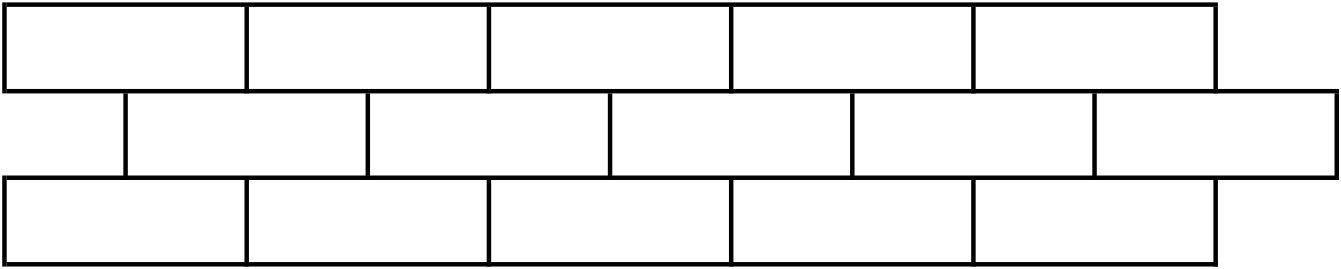
\includegraphics[width=0.6\textwidth]{Figures/01.png}
        \end{center}}
        \item[b.] {Có bao nhiêu cách chọn ra 4 viên gạch, mỗi viên từ một hàng trong hình sau đây, sao cho không có hai viên gạch nào được lấy ra nằm kề nhau?
        
        \begin{center}
            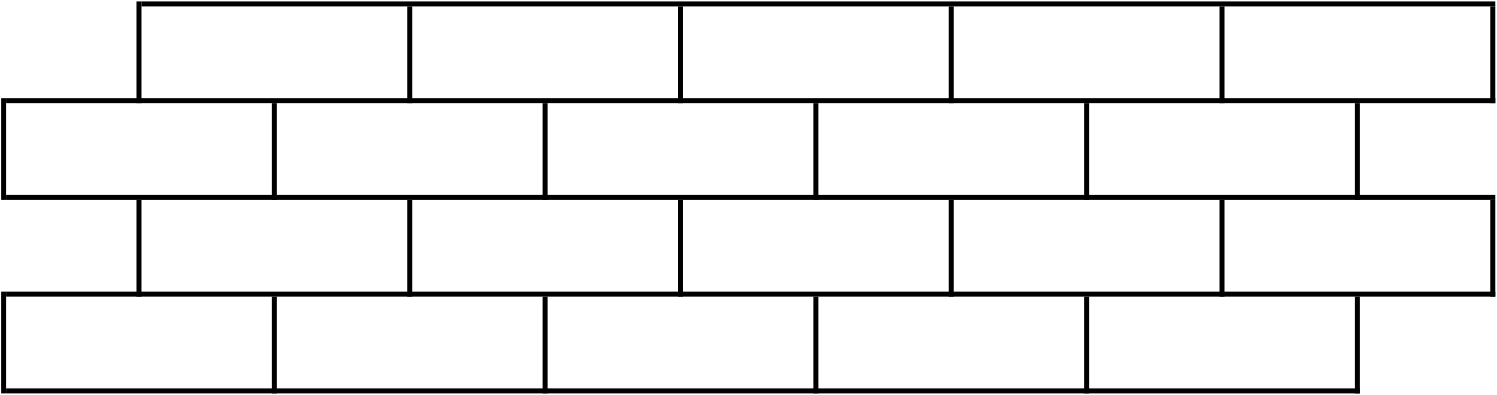
\includegraphics[width=0.6\textwidth]{Figures/02.png}
        \end{center}}
    \end{enumerate}

\paragraph{Analysis -- Phân tích bài toán} \mbox{} \\

Nhìn qua, ta thấy được đây là một bài tổ hợp, có thể tách ra thành bài toán con để giải quyết, rút ra nhận xét rằng bài toán đang hướng đến kỹ thuật quy hoạch động. \\

Theo đề bài, với 3 hàng ta cần đếm số cách chọn ra 3 viên gạch, với 4 hàng ta cần đếm số cách chọn ra 4 viên gạch.Vậy từ những dữ kiện trên, ta rút ra được bài toán tổng quát là xét $n$ hàng, mỗi hàng có $c$ viên gạch, đếm số cách chọn $n$ viên (mỗi hàng 1 viên) sao cho không có hai viên gạch nào được lấy ra nằm kề nhau. \\

Gọi $dp[n][c]$ là số cách chọn khi xét đến hàng thứ $n$, đang chọn viên gạch thứ $c$. Bài toán cơ sở là $dp[1][i] = 1$ - số cách chọn viên gạch thứ $i$ ở hàng $1$ luôn là $1$.\\

Do các hàng gạch chồng so-le nhau, để ý nếu xét hàng đầu là hàng thụt vào thì ở hàng chẵn, nếu ta chọn viên đầu tiên thì xét hàng trước đó ta luôn chọn được tất cả các viên ngoại trừ viên đầu hàng. Xét các viên gạch còn lại, chọn được tất cả các viên ở hàng trước ngoại trừ 2 viên: viên cùng chỉ số và viên có chỉ số ngay trước nó. \\

Ý tưởng cũng tương tự với hàng lẻ. \\

Kết quả bài toán: $\sum_{i =1}^{c}dp[n][i]$ - Số cách chọn là tổng số cách khi xét đến hàng $n$, ta chọn viên gạch thứ $i$.\\



\paragraph{Program -- Chương trình} \mbox{} \\


\begin{lstlisting}
#include <bits/stdc++.h>
using namespace std;

int main() {
	int n, c;
	cin >> n >> c;
	vector<vector<int>> dp(n + 1, vector<int>(c + 1, 0));
	for (int i = 1; i <= c; i++) {
		dp[1][i] = 1;
	}
	for (int i = 2; i <= n; i++) {
		for (int j = 1; j <= c; j++) {
			if (i % 2 == 1) {
				for (int brickInPreviousRow = 1; brickInPreviousRow <= c; brickInPreviousRow++) {
					if (brickInPreviousRow == j || brickInPreviousRow + 1 == j) {
						continue;
					}
					dp[i][j] += dp[i - 1][brickInPreviousRow];
				}
			}
			else {
				for (int brickInPreviousRow = 1; brickInPreviousRow <= c; brickInPreviousRow++) {
					if (brickInPreviousRow == j || brickInPreviousRow - 1 == j) {
						continue;
					}
					dp[i][j] += dp[i - 1][brickInPreviousRow];
				}
			}
		}
	}
	int ans = 0;
	for (int i = 1; i <= c; i++) {
		ans += dp[n][i];
	}
	cout << ans;
}
	
\end{lstlisting}
%------------------------------------------------------------------------------%

\section{Miscellaneous}

\subsection{Contributors}

\begin{enumerate}
	\item {\sc NGUYỄN QUẢN BÁ HỒNG - TEMPLATE}: \url{https://github.com/NQBH/advanced_STEM_beyond/blob/main/VMC/NQBH_VMC.tex}.
\end{enumerate}

%------------------------------------------------------------------------------%

\printbibliography[heading=bibintoc]
	
\end{document}